\documentclass[12pt,english,dvipsnames]{beamer}
\usepackage[mathletters]{ucs}
\usepackage[utf8x]{inputenc}
\usepackage{babel}
\usepackage{xcolor}
\usepackage{listings}
\usepackage{textcomp}
\usepackage[noBBpl]{mathpazo}
\usepackage{courier}
\usepackage{fancyvrb}
\usepackage{amsmath}
\usepackage{amssymb}
\usepackage{url}

\usecolortheme{crane}
\usefonttheme{serif}

\usepackage{tikz}
\usetikzlibrary{arrows,calc,shapes,chains}

\newcommand{\K}{\mathbb{K}}  % Biot-Savart kernel
\newcommand{\R}{\mathbb{R}}  % set of real numbers
\renewcommand{\vec}{\mathbf}
\newcommand{\x}{\vec x}      % position
\newcommand{\vel}{\vec u}    % velocity
\DeclareMathOperator{\divergence}{div}
\DeclareMathOperator{\curl}{curl}
\DeclareMathOperator{\supp}{supp}
\providecommand{\abs}[1]{\lvert#1\rvert}
\providecommand{\norm}[1]{\lVert#1\rVert}
\newcommand{\pd}[2]{\frac{\partial #1}{\partial #2}}
\newcommand{\md}[2]{\frac{D#1}{D#2}}
\newcommand{\od}[2]{\frac{d#1}{d#2}}

\title{GPU-accelerated simulation of a Lamb--Oseen vortex
using 2-D Vortex Methods}
\author{Roberto Bonvallet}
\date{March 28th, 2011}

\begin{document}
  \begin{frame}
    \maketitle
  \end{frame}

  \begin{frame}
    \frametitle{Fluid Dynamics}
    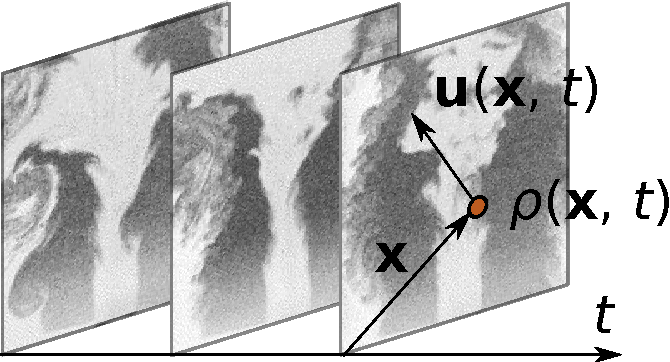
\includegraphics{fluid1.pdf}
  \end{frame}

  \begin{frame}
    \frametitle{Eulerian methods}
    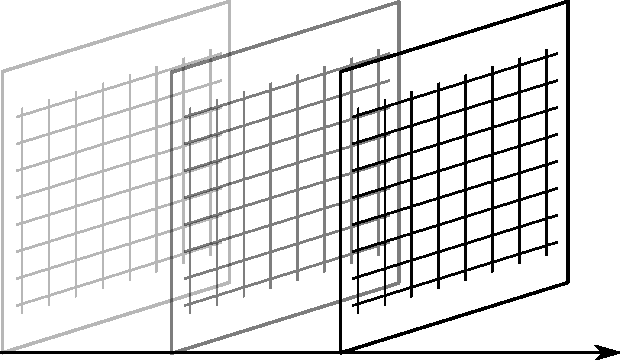
\includegraphics{fluid2.pdf}
  \end{frame}

  \begin{frame}
    \frametitle{Lagrangian methods}
    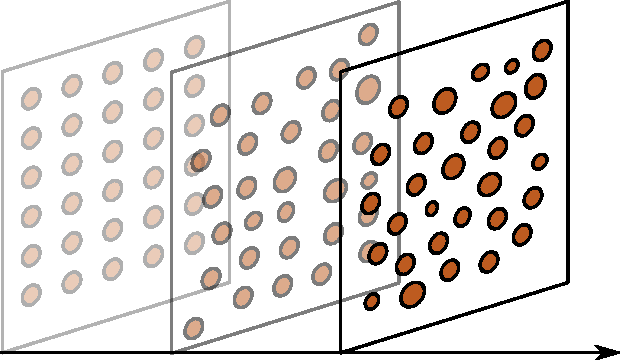
\includegraphics{fluid3.pdf}
  \end{frame}

  \begin{frame}
    \frametitle{Fluid equations in Eulerian coordinates}
    \begin{itemize}
      \item Continuity equation:
        \begin{equation}
          \pd{ρ}{t} + ∇\cdot(ρ\vel) = 0
        \end{equation}
      \item Navier-Stokes equations:
        \begin{equation}
          ρ\left(\pd{\vel}{t} + \vel\cdot∇\vel\right) = -∇p + μ\,Δ\vel + \vec{f}
        \end{equation}
    \end{itemize}
  \end{frame}

  \begin{frame}
    \frametitle{Fluid equations in Lagrangian coordinates}
    \begin{itemize}
      \item Continuity equation:
        \begin{equation}
          \md{ρ}{t} = -ρ\divergence\vel
        \end{equation}
      \item Navier-Stokes equations:
        \begin{equation}
          ρ\md{\vel}{t} = -∇p + μ\,Δ\vel + \vec{f}
        \end{equation}
    \end{itemize}
  \end{frame}

  \begin{frame}
    \frametitle{Turbulence}
    \begin{center}
      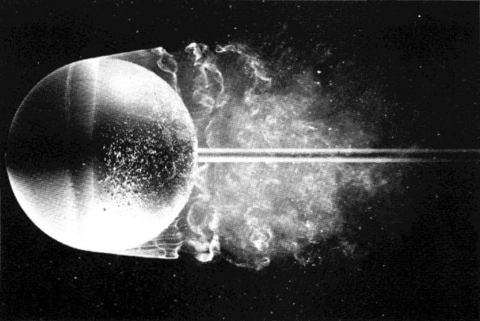
\includegraphics[scale=.9]{flow-past-sphere.jpg}
    \end{center}
  \end{frame}

  \begin{frame}
    \frametitle{Vorticity}
    \begin{center}
      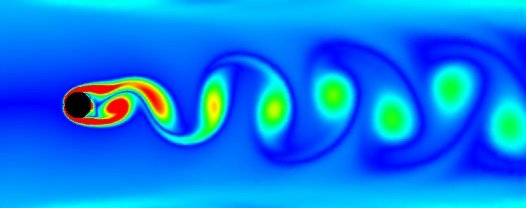
\includegraphics[scale=.6]{cylinder-vorticity.jpg}
    \end{center}

    \[ \mathbold\omega = ∇\times\vel = \frac{dΓ}{dA} \]
  \end{frame}

  \begin{frame}
    \frametitle{2-D Vortex Methods}
    \begin{itemize}
      \item Incompressible flow:
        \begin{itemize}
          \item  \(∇\cdot\vel = 0\);
          \item continuity equation reduces to \(\displaystyle\md{ρ}{t} = 0\).
        \end{itemize}
      \item Velocity-vorticity formulation of N-S eqs.:
        \begin{align}
          ρ\md{\vel}{t} &= -∇p + μ\,Δ\vel \\
          ρ\md{ω}{t}    &= μ\,Δω \\
          \md{ω}{t}    &= ν\,Δω
        \end{align}
    \end{itemize}
  \end{frame}

  \begin{frame}
    \frametitle{2-D Vortex Methods}
    \begin{align}
      \md{ω}{t} &= ν\,Δω \\
      \divergence\vel &= 0 \\
      \curl\vel &= \mathbold\omega \\
      ω(\,\cdot\,, 0) &= ω_0
    \end{align}
  \end{frame}

  \begin{frame}
    \frametitle{Recovery of velocity}
    \begin{itemize}
      \item Velocity field recovered by solving Poisson's equation:
        \begin{equation}
          \left.
          \begin{split}
            \divergence\vel &= 0 \\
            \curl\vel &= \mathbold\omega
          \end{split}
          \right\}\;\Longrightarrow\;
          Δ\vel = -\curl\mathbold\omega
        \end{equation}
      \item Biot-Savart law:
        \begin{align}
          \vel(\x, t) &=
            \int\bigl(\curl\vec{G}\bigr)(\x - \x')\,ω(\x', t)\,d\x' \\
          \vel &= \K * ω,
            \quad\text{where \(\textstyle\K(x, y) = \frac{1}{2π\norm{\x}^2}(-y, x)\)}
        \end{align}
    \end{itemize}
  \end{frame}

  \begin{frame}
    \frametitle{Vortex Point Method}
    \begin{itemize}
      \item Domain discretized as a set of particles.
      \item Approximation of the vorticity field:
        \begin{equation}
          ω^h(x, t) \approx\sum_p α_p δ\bigl(\x - \x^h_p(t)\bigr)
        \end{equation}
      \item Velocity restored by Biot-Savart law
    \end{itemize}
  \end{frame}

  \begin{frame}
    \frametitle{Vortex Blob Method}
    \begin{itemize}
      \item Smooth cutoff function \(ζ\) such that \(\int ζ(\x)\,d\x = 1\).
      \item Mollified particle: \(ζ_ε(\x) = ε^{-2} ζ(\x/ε)\).
      \item Mollified kernel:   \(\K_ε = \K * ζ_ε\).
      \item Numerical method:
        \begin{align}
          \od{\x^h_p}{t} &= \vel^h(\x^t_p, t) \\
          \od{ω^h_p}{t}    &= ν\,Δω^h_p
        \end{align}
        with \(\vel^h = \K_ε * ω^h\).
    \end{itemize}
  \end{frame}

  \begin{frame}
    \frametitle{Lamb-Oseen vortex}
    \begin{equation}
      ω(r, t) = \frac{Γ_0}{4πνt} \exp(-r^2/4νt)
    \end{equation}
    \includegraphics[scale=.45]{lamb-oseen-vorticity.pdf}
  \end{frame}

  \begin{frame}
    \frametitle{Lamb-Oseen vortex velocity field}
    \begin{align}
      u_\theta(r, t) &= \frac{Γ_0}{2πr} \bigl(1 - \exp(-r^2/4νt)\bigr) \\
      \vec{u} &= (-y, x)\cdot u_\theta(r, t)/r
    \end{align}
    \includegraphics[scale=.30]{lamb-oseen-velocity.pdf}
  \end{frame}

  \begin{frame}
    \frametitle{Wingtip vortices as Lamb-Oseen vortices}
    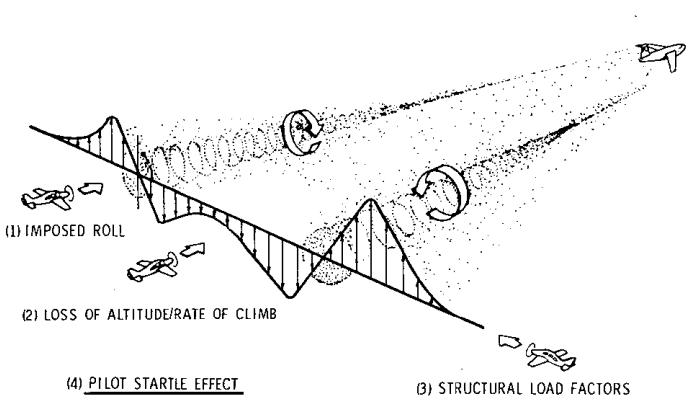
\includegraphics[scale=.45]{wingtip-vortices.png}
  \end{frame}

  \begin{frame}
    \frametitle{}
    \begin{figure}
      \centering
      \tikzstyle{vm-block}=[draw]
      \tikzstyle{vm-arrow}=[->,thick]
      \tikzstyle{vm-block-o}=[draw,fill=blue!15]
      \begin{tikzpicture}[node distance=5ex]
        \node[vm-block]   (disc)                 {Discretization};
        \node[vm-block]   (vel)  [below of=disc] {Velocity evaluation};
        \node[vm-block]   (conv) [below of=vel]  {Convection};
        \node[vm-block]   (diff) [below of=conv] {Diffusion};
        \node[vm-block-o] (bc)   [below of=diff] {Satisfaction of BCs};
        \node[vm-block-o] (spa)  [below of=bc]   {Spatial adaption};
        \node[vm-block-o] (fs)   [right of=vel, node distance=12em] {Fast summation};
        \node[vm-block-o] (mf)   [right of=bc,  node distance=12em] {Measurement of forces};
        \draw[vm-arrow] (disc) to (vel);
        \draw[vm-arrow] (vel)  to (conv);
        \draw[vm-arrow] (conv) to (diff);
        \draw[vm-arrow] (diff) to (bc);
        \draw[vm-arrow] (bc)   to (spa);
        \draw[vm-arrow, dashed] (fs)   to (vel);
        \draw[vm-arrow, dashed] (bc)   to (mf);
        \draw[vm-arrow] (spa.west) to [out=180,in=180] (vel.west);
      \end{tikzpicture}
      \label{fig:vm-blocks}
      \caption[Builiding blocks of a viscous Vortex Method]{
        Basic building blocks of a viscous Vortex Method implementation,
        as described in [Barba04].}
    \end{figure}
  \end{frame}

  \begin{frame}
    \frametitle{Velocity evaluation}
    \begin{align}
      ω^h_ε  &= \sum_p α_p  ζ_ε(\x - \x^h_p) \\
      \vel^h &= \sum_p α_p \K_ε(\x - \x^h_p)
    \end{align}
  \end{frame}

  \begin{frame}
    \frametitle{Trajectory integration}
    \begin{itemize}
      \item Velocity evaluation:
        \begin{equation}
          \vel^h = \sum_p α_p \K_ε(\x - \x^h_p)
        \end{equation}
      \item Time-stepping:
        \begin{equation}
          \x_p^{(n + 1)} = \x_p^{(n)} + \vel_p^{(n)}\cdot δt
        \end{equation}
    \end{itemize}
  \end{frame}

  \begin{frame}
    \frametitle{Diffusion model}
    \begin{itemize}
      \item Diffusion equation:
        \begin{equation}
          \od{ω^h_p}{t} = ν\,Δω^h_p
        \end{equation}
      \item Particle-Strength Exchange:
        \begin{align}
          Δ_ε ω(\x) &= ε^{-2} \int [ω(\x') - ω(\x)]\cdot η_ε(\x' - \x)\,d\x' \\
          Δ_ε ω_p &= ε^{-2} \sum_q v_q [ω_q^h - ω_p^h]\cdot η_ε(\x_q - \x_p) \\
          Δ_ε α_p &= ε^{-2} \sum_q [α_q^h - α_p^h]\cdot η_ε(\x_q - \x_p) \\
          \dot{α}_p &= νε^{-2} \sum_q [α_q^h - α_p^h]\cdot η_ε(\x_q - \x_p)
        \end{align}
    \end{itemize}
  \end{frame}

  \begin{frame}
    \frametitle{Diffusion integration}
    \begin{itemize}
      \item Evaluation of \(\dot{α}\):
        \begin{equation}
          \dot{α}_p = νε^{-2} \sum_q [α_q^h - α_p^h]\cdot η_ε(\x_q - \x_p)
        \end{equation}
      \item Time-stepping:
        \begin{equation}
          α_p^{(n + 1)} = α_p^{(n)} + \dot{α}_p^{(n)}\cdot δt
        \end{equation}
    \end{itemize}
  \end{frame}

  \begin{frame}
    \frametitle{GPU solver}
    Problem to be solved:
    \begin{align}
      x_p^{(n + 1)} &= x_p^{(n)} + u_p^{(n)}\, δt, \\
      y_p^{(n + 1)} &= y_p^{(n)} + v_p^{(n)}\, δt, \\
      α_p^{(n + 1)} &= α_p^{(n)} + \dot{α}_p^{(n)}\, δt.
    \end{align}
    with
    \begin{align}
        %\label{eq:evaluation}
        (u_p, v_p) &= \sum_q \vec{U}_{pq},   & \vec{U}_{pq} &= α_p \K_ε(\x_p - \x_q) \\
        \dot{α}_p  &= νε^{-2} \sum_q A_{pq}, &       A_{pq} &= [α_q - α_p]\,η_ε(\x_p - \x_q).
    \end{align}
  \end{frame}

\tikzstyle{innergrid}=[gray!80]
\tikzstyle{tile}=[green!60!black, thick]
\tikzstyle{sync}=[red!60!black, thick, dashed]
\tikzstyle{thread}=[->, decorate, decoration={snake, amplitude=.6}]
\tikzstyle{examplecell}=[fill=orange, opacity=.5]
\tikzstyle{kernelcall}=[#1, rounded corners=2pt, very thick, pattern color=#1]
\tikzstyle{kernelarrow}=[->, thick, out=90, in=180]
\tikzstyle{imglabel}=[anchor=west, text opacity=1.0, fill=white, fill opacity=.5,
                      text height=1ex, text depth=.25ex, rounded corners]
\tikzstyle{row}=[fill=yellow!50!white]
\def\N{43}

  \begin{frame}
    \begin{tikzpicture}[scale=.14, yscale=-1, font=\small]
      \only<1> {
        \def\myX{25.5}
        \def\myY{39.5}
        \fill[row] (0, \myY - .5) rectangle ++(\N, 1);
        \draw[innergrid] (0, 0) grid ++(\N, \N);
        \draw[tile] (0, 0) rectangle ++(\N, \N);
        %\foreach \i in {0,...,44}
        %  \node[anchor=east, font=\tiny] at (0, \i + .5) {\i};
        %\foreach \j in {0,...,44}
        %  \node[anchor=west, font=\tiny, rotate=90] at (\j + .5, 0) {\j};
        \draw (-1, \myY) -- (\myX, \myY);
        \draw (\myX, -1) -- (\myX, \myY);
        \node [draw, red!80!black, very thick, circle, inner sep=.5ex] (interaction) at (\myX, \myY) {};
        \node at (-2, \myY) {\(p\)};
        \node at (\myX, -2) {\(q\)};

        \draw (44.5, 10) node[imglabel, anchor=west] (interaction eq) {
          \(
           \left\{
           \begin{aligned}
             {\vec U}_{pq} &= α_q\,\K_ε(\x_p - \x_q) \\
             A_{pq}        &= [α_q - α_p]\,η_ε(\x_p - \x_q) \\
           \end{aligned}
           \right.
          \)
        };
        \draw[red!80!black, very thick, ->, out=-45, in=180] (interaction) to (interaction eq.west);

        \draw (44.5, \myY) node[imglabel, anchor=west] (total eq) {
          \(
           \begin{aligned}
             (u_p, v_p) &= \phantom{νε^{-2}}\sum_q \vec{U}_{pq} \\
             \dot{α}_p  &=          νε^{-2} \sum_q A_{pq}
           \end{aligned}
          \)
        };
      }

      \only<2-> {
        \foreach \block in {0,1,...,6} {
          \draw[innergrid] (0, \block * 9) grid      ++(\N, 8);
          \draw[tile]      (0, \block * 9) rectangle ++(\N, 8);
          \node[anchor=east] at (-4, 9 * \block + 4) {block \block};
          \foreach\thread in {0,...,7} {
            \node[anchor=east, font=\Tiny] at (0, 9 * \block + \thread + .5) {\thread};
          }
        }
      }

    \end{tikzpicture}
  \end{frame}

  \begin{frame}
    \frametitle{Work distribution}
    \begin{itemize}
      \item one particle \(\longrightarrow\) one thread
      \item each thread evaluates all the terms
        of the formulas for the derivatives
        for one particle
      \item \(N^2\) interactions \(\longrightarrow\)
        \(N\) threads \(\times\) \(N\) particle-particle evaluations
      \item synchronization and data fetch between tiles
    \end{itemize}
  \end{frame}

  \begin{frame}
    \centering
    \includegraphics[scale=.7, viewport=120 200 800 650]{work.pdf}
  \end{frame}

  \begin{frame}
    \frametitle{Memory management}
    \begin{itemize}
      \item Global array of particles
      \item \((x_p, y_p, α_p)\) stored as \texttt{float4}
        \begin{itemize}
          \item exploits coalescing and alignment
        \end{itemize}
      \item Subset of particles
        are loaded to shared memory
        at synchronization points
    \end{itemize}
  \end{frame}

  \begin{frame}
    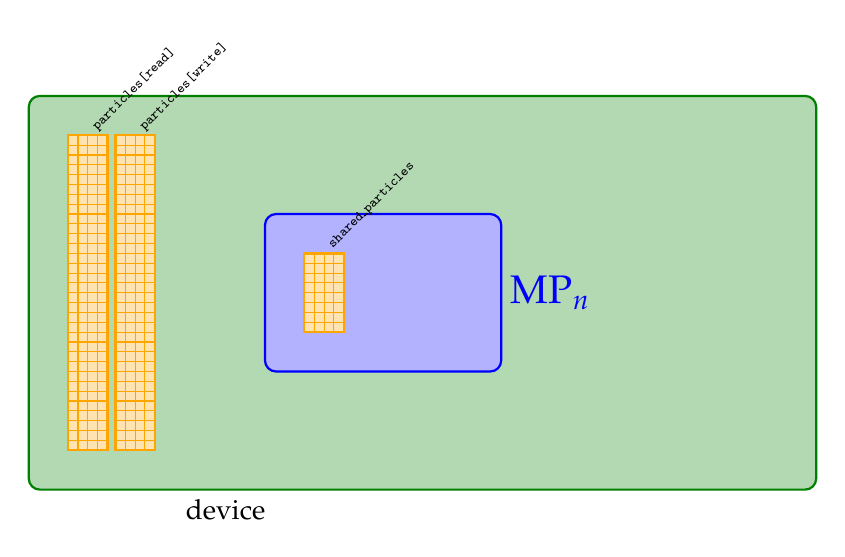
\begin{tikzpicture}[scale=.5, yscale=-1]
      \begin{scope}
        \draw[thick, Green, fill=Green!30, rounded corners] (0, 0) rectangle (20, 10);
        \node[anchor=north] at (5, 10) {device};
        \foreach \i/\dx/\what in {0/1cm/read, 1/2.2cm/write} {
          \begin{scope}[xshift=\dx, yshift=1cm]
            \draw[thick, Orange, fill=Orange!30] (0, 0) rectangle ++(1, 8);
            \draw[thin,  Orange, step=0.25cm]    (0, 0) grid      ++(1, 8);
            \node[rotate=45, anchor=west, font=\tiny] at (0.5, 0) {\texttt{particles[\what]}};
          \end{scope}
        }
        \begin{scope}[xshift=6cm, yshift=3cm]
          \draw[thick, Blue, rounded corners, fill=Blue!30] (0, 0) rectangle (6, 4);
          \node[font=\Large, Blue, anchor=west] at (6, 2) {MP\(_n\)};
          \draw[thick, Orange, fill=Orange!30] (1, 1) rectangle ++(1, 2);
          \draw[thin,  Orange, step=0.25cm]    (1, 1) grid      ++(1, 2);
          \node[rotate=45, anchor=west, font=\tiny] at (1.5, 1) {\texttt{shared\_particles}};
        \end{scope}

      \end{scope}
    \end{tikzpicture}
  \end{frame}

  \begin{frame}
    \centering
    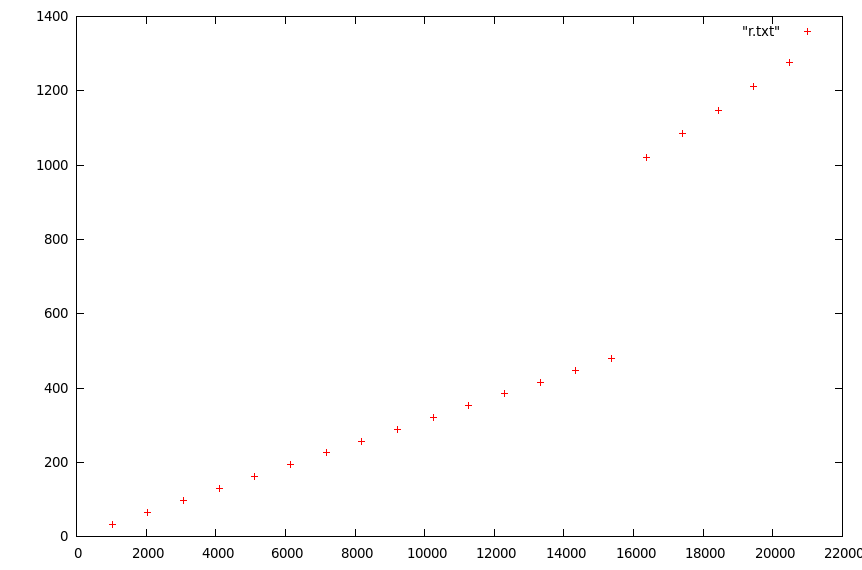
\includegraphics[scale=.35]{execution-time.png}
  \end{frame}

\end{document}
